\section{Results}
\label{sec:results}
Resultater vi skal ha med
\begin{itemize}
\item $\beta$ - confidens intervall
\item MSE - train vs test (OLS)
\item R2 - train vs test (OLS)
\item Bias-variance tradeoff (OLS)
\item Ridge - beste $\lambda$ og degree
\item Lasso - beste $\lambda$ og degree
\item tabell minste feil for de ulike metodene
\item Terrengdata - OLS
\item Terrengdata - Ridge
\item Terrengdata - Lasso
\item Tabell - minste feil for de ulike metodene
\end{itemize}
\subsection{Regression on Franke's function}
The {''}terrain'' data $z$ in this part was produced by applying Franke's function to a $n\cross n$ evenly spaced $xy$ grid, with $x_i,y_i\in [0,1]$, and for each point add a normally distributed noice with $\mu = 0$ and $\sigma^2 = 0.1$.
\subsubsection{$\beta$-values confidence interval}
Before applying any resampling methods we used the regular \emph{ordinary least squares} method \eqref{eq:ols} to our data and had a look at the confidence interval of the $\beta$ values when approximating the data to a polynomial of degree $m=5$. The confidence intervals are shown in figure \ref{fig:betaconfidence}.

\begin{figure}[htbp]
	\centering
	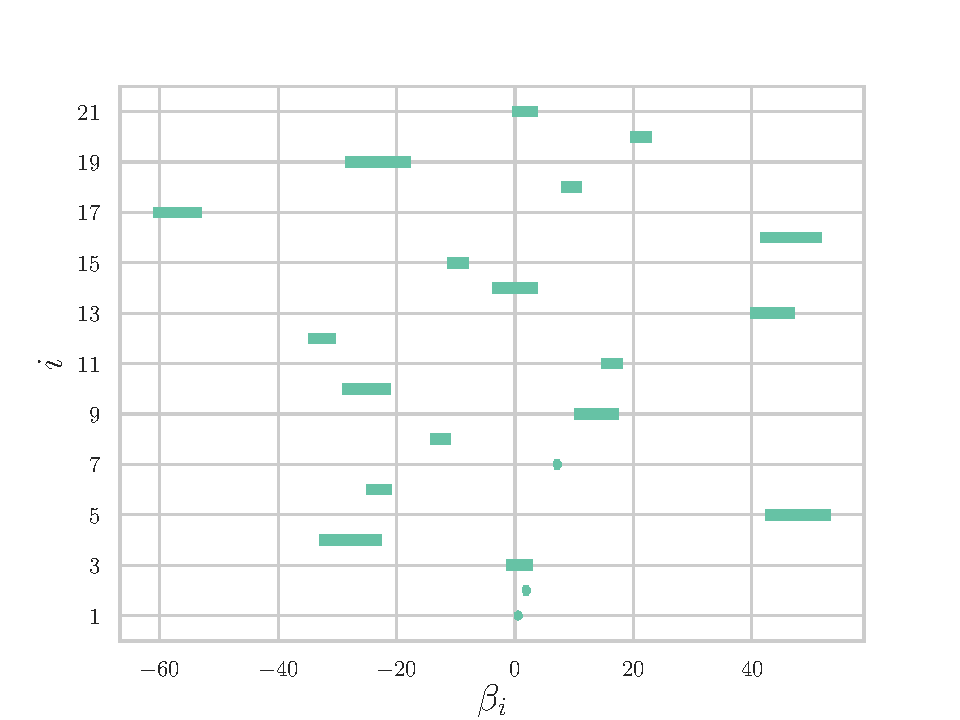
\includegraphics[width=0.5\textwidth]{betaconfidence}
	\caption{DENNE FIGUREN SKAL ENDRES. The $\beta$-values and their confidence interval for $n=??$ and $m=5$ with OLS.}
	\label{fig:betaconfidence}
\end{figure}

\subsubsection{MSE and $R^2$ of OLS, with and without resampling}
To study the mean squared error \eqref{eq:mse} as a function of the model complexity, we applied the OLS-method to the data set for various values of polynomial degree $m$, both when using the entire data set as both test and training data, and by using the bootstrap method (algorithm \ref{alg:bootstrap}) for resampling (figure \ref{fig:mseVSdegreeOLS}).

% Eksempel for figurer
\begin{figure}[htbp]
	\centering
	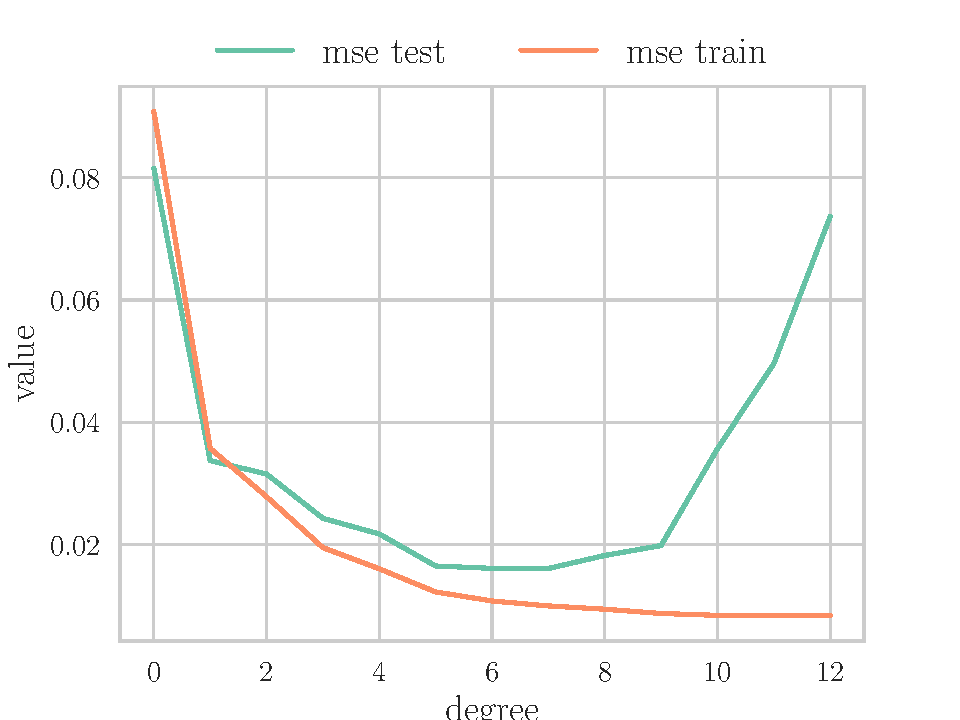
\includegraphics[width=0.5\textwidth]{mseVSdegreeOLS}
	\caption{MSE of the model as a function of degree $m$, with n=20, noice $\sigma^2$ = 0.1. In the case where no resampling is done (mse-train), the MSE flattens out at a low value. When applying the bootstrap method (mse-test) for resampling however, the MSE begins to rise after reaching a certain model complexity, creating a minimum point where the error is the lowest.}
	\label{fig:mseVSdegreeOLS}
\end{figure}

Applying the same analisys to the $R^2$-score \eqref{eq:r2} of the two cases, we get the result as shown in figure \ref{fig:r2VSdegreeOLS}. For the $R^2$ score, we found the results easier to obtain when using the \emph{k-fold cross validation} method (algorithm \ref{alg:k-fold}) for resamling.
\begin{figure}[htbp]
	\centering
	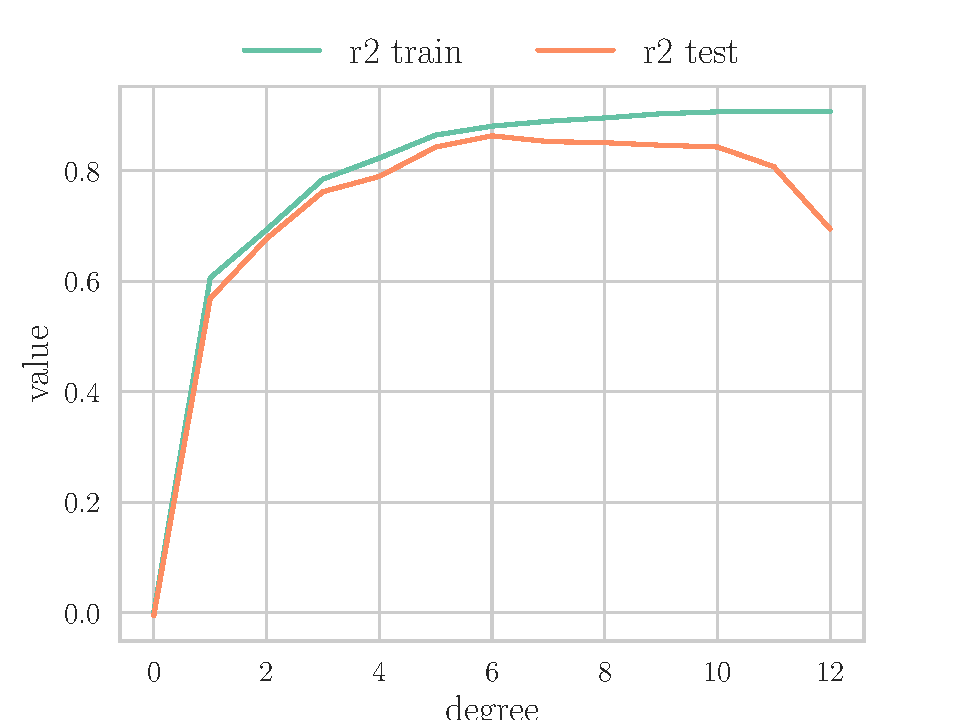
\includegraphics[width=0.5\textwidth]{r2VSdegreeOLS}
	\caption{$R^2$-score of the model as a function of degree $m$, with n=20, noice $\sigma^2$ = 0.1. In the case where no resampling is done (r2-train), the $R^2$ increases and then flattens out. When applying the k-fold cross validation method (r2-test) for resampling however, the $R^2$ begins to decrease after reaching a certain model complexity, creating a maximum point where the $R^2$-score is closest to 1 (the optimal value).}
	\label{fig:r2VSdegreeOLS}
\end{figure}

\subsubsection{Bias-Variance-tradeoff}

\vfill
\newpage
